\documentclass[hyperref=unicode,graphics=pdflatex,13pt]{beamer}

\mode<presentation>
{
  \usetheme{default}
%  \usecolortheme{crane}
  \setbeamercovered{invisible}
  \setbeamertemplate{footline}{\hfill\insertframenumber/\inserttotalframenumber}
  \setbeamersize{text margin left=0.4cm,sidebar width left=0cm}
}

\graphicspath{{pic/}}

\usepackage[utf8]{inputenc}
\usepackage[T2A]{fontenc}
\usepackage[english, russian]{babel}
\usepackage{times}
\usepackage{color, colortbl}
\definecolor{res}{RGB}{255, 215, 0}
\definecolor{olivegreen}{RGB}{38, 141, 38}
\usepackage{xspace}
\usepackage{tabularx}
\usepackage{listings}

\beamertemplatenavigationsymbolsempty
%\setbeamerfont{page number in head/foot}{size=\HUGE}


\title[Dishonest Casino Problem\ldots]{Solving Dishonest Casino Problem \\ With Evolutionary Algorithms}

\author[\mbox{V. Mironovich, D. Antipov, V. Volochay}]
{V. Mironovich \and D. Antipov \and V. Volochay}
\institute[Университет ИТМО]{{
\includegraphics[height=0.2\textwidth]{pic/itmo-dots-en-small.pdf}}\\~\\~Saint-Petersburg, Russia}
\date[June 4]{June 4, 2015}

% NOTE: I HATE USELESS TOCS
%\AtBeginSection[] {
%  \begin{frame}<beamer>{}
%    \tableofcontents[currentsection]
%  \end{frame}
%}

\begin{document}

\begin{frame}[noframenumbering,plain]
  \titlepage
\end{frame}

% NOTE
%\begin{frame}[noframenumbering,plain]
%  \tableofcontents
%\end{frame}

\section{Introduction}

% NOTE
%subsection too much
%\subsection{Dishonest Casino Problem}
\begin{frame}{Original Dishonest Casino Problem}
\begin{itemize}
   \item Casino uses two dices
   \item One is fair, the other one is weighted to produce more sixes
   \item Casino switches the dices at unknown times
   \item We know probabilities for Markov process and dice distributions
   \item Detect switch times
\end{itemize}

\centering{Solved with DynProg or previosly reported algorithms.}
\end{frame} 

\begin{frame}{Proposed statement of DCP}
 \begin{itemize}
  \item Still the same two dices
  \item We know nothing about probabilities and distributions
  \item The underlying process is still the same
  \item Detect switch times
  \end{itemize}

\end{frame}

% NOTE: Somethign something
%\begin{frame}{Group work process}
% \begin{itemize}
%  \item Everyone worked on his own solution
%  \item Exchanging ideas and suggestions
% \end{itemize}
%\end{frame}


\section{Solution} %kay m8 
\begin{frame}{Solution}
  \begin{itemize}
   \item Let's try something with evolutionary algorithm
   \item Why? Because we can...probably
   \item Logic from evolution in nature
   \item $\rightarrow$ Represent individual \\ $\hookrightarrow$ Mutate and Reproduce \\
   $\hookrightarrow$ Optimize fitness function \rotatebox[origin=c]{-180}{$\hookrightarrow$} \\ $\hookrightarrow$ Assume the best as the answer
  \end{itemize}

\end{frame}

\begin{frame}{Evolutionary algorithm}
 \begin{itemize}
  \item Generate a binary vector $S$ and assume:
   \begin{itemize}
   \item $S_t = 0$, if $X_t$ was given by first generator
   \item $S_t = 1$, if $X_t$ was given by second generator
   \end{itemize}
  \item Mutation: flipping random bit
  \item Crossover: single-point exchange of tails
 \end{itemize}
\end{frame}

\begin{frame}{Choosing fitness}
\begin{itemize}
   \item Minimize the average deviation of $p(S_i=s | X_i = x)$ calculated by the Bayes theorem from this probabilities calculated by assumption vector
   \item Maximize the Bhattacharyya distance beetween the sourse distributions:
   $$D_B(p, q) = -\ln{\sum_{\omega \in \Omega} \sqrt{p(\omega)q(\omega)}}$$
   \item %TODO: Tut Vika rasskazhet pro Kolmagorova
\end{itemize}

\end{frame}

\section{Failures 1}
\begin{frame}{Failures: Conditional probability}
 \begin{itemize}
  \item We can get distributions of the generators using assumption
  \item Calculate the conditional probabilities using Bayes Theorem:
  $$p(S_t = s | X_t = x) = \frac{p(X_t = t | S_t = s) p(S_t = s)}{\sum_{i \in \{0, 1\}}p(X_t = t | S_t = i) p(S_t = i)}$$
  \item Compare to conditional probabilities using assumption:
  $$p(S_t = s | X_t = x) = \frac{count(t: X_t = x \wedge S_t = s)}{count(t: X_t = x)}$$
  \item Minimize an avarage sqare deviation
  \item It doesn't give good results because it actually minimizes the deviation of generators. But in original problem usual dice have quite big deviation.
 \end{itemize}

\end{frame}

\begin{frame}{Failures: Bhattacharyya distance}
\begin{itemize}
 \item Bhattacharyya distance is prone to overfitting. Falls into making two generators ``absolutely distinct'' and the distance equal to $\infty$
 \item Try to force the equality of generators' domains by making $p(x) = max(1/len(S), p(x_i))$
 \item Works better but still overfits
\end{itemize}
\end{frame}

\begin{frame}{Overfitting}
 %TODO overfitting example
  \begin{itemize}
   \item Length = 100, (0.5, 0.5) probabilities
   \begin{itemize}
   \item distance of original 2.01, distance of found 3.24
   \item Guessed: 24 out of 44, 54.5\%
   \item Wrong: 25 out of 49, 51\%
   \end{itemize}
  \item Length = 100, (0.9, 0.35) probabilities
  \begin{itemize}
   \item distance of original 1.60, distance of found 3.22
   \item Guessed: 12 out of 25, 48.0\%
   \item Wrong: 39 out of 51, 76\%
  \end{itemize}
  \end{itemize}
\end{frame}

\begin{frame}{Overfitting}
 \begin{itemize}
  \item Assume we know Bhattacharyya distance for our sequence
  \item Optimize to it ($ abs(bchd(S)-actual) $
 %TODO example here
  \item Length = 100, (0.5, 0.5) probabilities
  \begin{itemize}
   \item Guessed: 27 out of 52, 51.92307692307692\%
   \item Wrong: 34 out of 61, 55\%
  \end{itemize}
  \item Length = 100, (0.9, 0.35) probabilities
  \begin{itemize}
   \item distance of original 1.77, distance of found 1.82
   \item Guessed: 6 out of 25, 24.0\%
   \item Wrong: 38 out of 44, 86\%
  \end{itemize}
  \item Questionable
  \end{itemize}
\end{frame}

%TODO Assuming that kolmogorov is shitty too, insert something here


\section{Current ideas in work}
%TODO recent for calling my work shit
\subsection{Sliding windows}
\begin{frame}{One sliding window}
\begin{itemize}
   \item Assume that we know the probability of switching beetween generators
   \item Choose the length of the window equal to the expected length of non-switching subsequence of $S$
   \item We can calculate the expectation of the in-window sequence for every window position
   \item It gives us nothing even after smoothing the expectations:
   \end{itemize}
   \begin{tabular}{cc}
      Without smoothing & With smoothing \\
      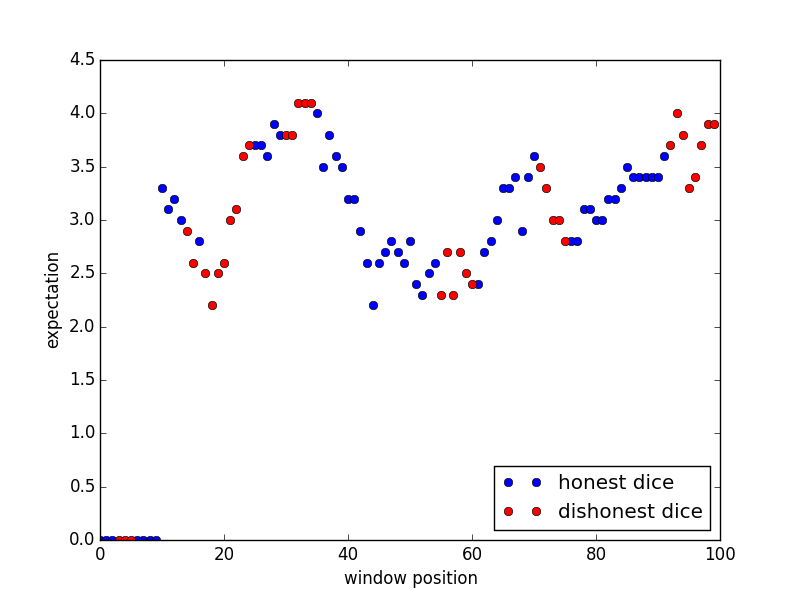
\includegraphics[width=5cm]{window_expectations.png} &
      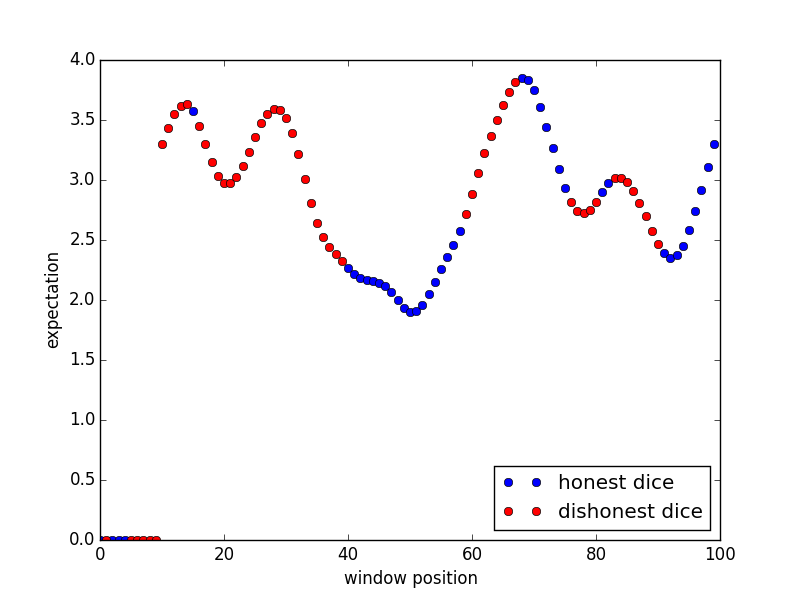
\includegraphics[width=5cm]{window_expectations_smoothed.png}
   \end{tabular}


\end{frame}

\begin{frame}{One sliding window}
\begin{itemize}
   \item Basing on calculated expectations we can try to assume that expectations of sources are the max and min expectation
   \item With this assumption we can try to find probabilities of each source on every step:
   \footnotesize$$p(S_t = 0 | X_t = x) = p(S_{t - 1} = 0) p(switch | X_t = x) +$$
   $$+p(S_{t - 1} = 1) (1 - p(switch | X_t = x))$$
   $$p(switch | X_t = x) = \frac{p(X_t = x| switch) * p(switch)}{p(X_t = x)}$$
   \footnotesize$$p(X_t = x| switch) = p(X_t = x | S_t = 0) * p(S_{t - 1} = 1) + $$
   $$+p(X_t = x | S_t = 1) * p(S_{t - 1} = 0)$$
   $$p(X_t = x | S_t = 0) = \frac{p(S_t = 0 | X_t = x)p(X_t = x)}{sum_{x} p(S_t = 0 | X_t = x}$$
   $$p(S_t = 0 | X_t = x)$$
   \item May be different assumptions about last probability. For example $$p(S_t = 0 | X_t = x) = \frac{1}{1 + a^{|x - E_{min}| - |x - E_{max}|}}$$
\end{itemize}
\end{frame}

\begin{frame}{One sliding window}
 But it doesn't work!
 
 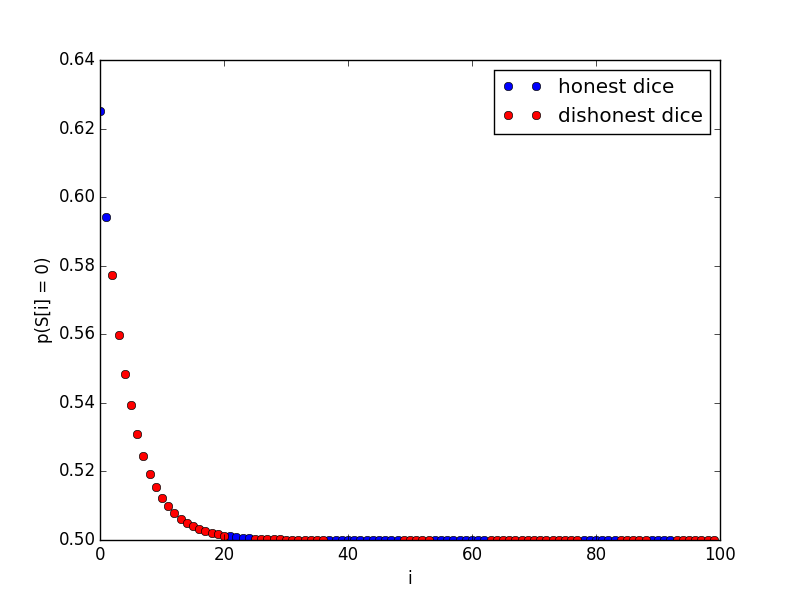
\includegraphics[width = 10cm]{one_window_probabilities.png}
\end{frame}


\begin{frame}{Two Sliding Windows}
\begin{itemize}
   \item Two sliding windows without interval between them
   \item Check the difference between them:
   \begin{itemize}
      \item difference of expectations
      \item Bhattacharyya distance
   \end{itemize}
   \item Nothing of it correlates with the real $S$:
\end{itemize}
\begin{tabular}{cc}
 Expectations & Bhattacharyya \\
 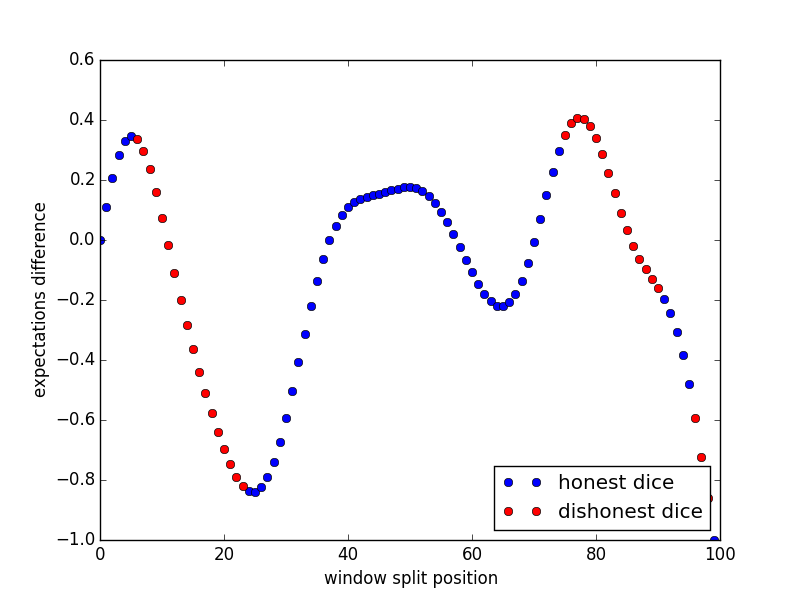
\includegraphics[width = 5cm]{two_windows_expectation.png} &
 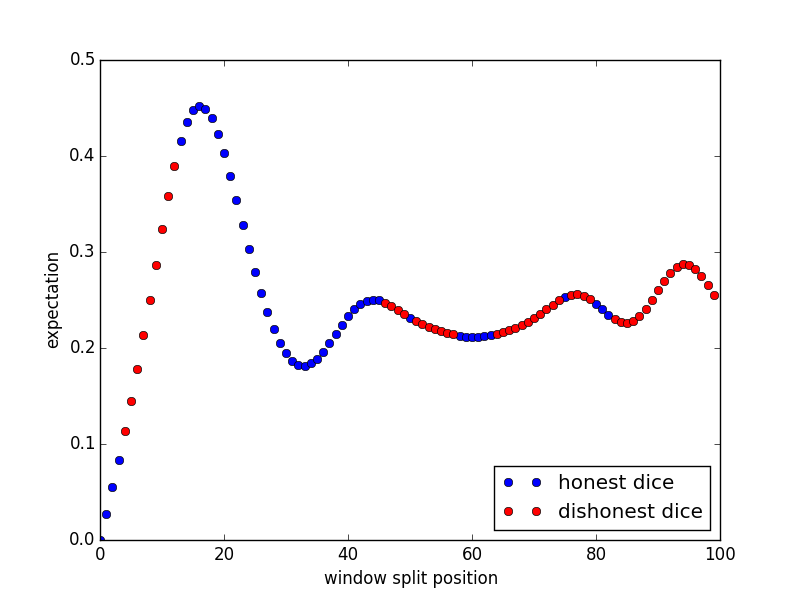
\includegraphics[width = 5cm]{two_windows_bhattacharyya.png}
\end{tabular}
\end{frame}

\subsection{Produce minimum number of values}
\begin{frame}{Minimum number of emissions}
 \begin{itemize}
  \item Assume we have a number of minimum generations for generator, before it can switch
  \item Assume we know that number
  \item Still optimizing as before
 \end{itemize}
\end{frame}

\begin{frame}[fragile]{So what?}
 \begin{itemize}
  \item Helps keeping number of switches close to the original
  \item But does not really work
\item Error piles up
\item Correctly shows which generator produced the number in sequence in 75\% of cases
 \end{itemize}

 \tiny\begin{lstlisting}
0...00011...111000...00011...1100000...000111111000000000...0000111111111
0...01111...110000...00111...1111000...000111111111111000...0000000000001
 \end{lstlisting}
\end{frame}

\subsection{Whatever Vika is doing}
%TODO may swap places in presentation

\section{Conclusion} %\sextion lololo

\begin{frame}{Conclusion}
 \begin{itemize}
  \item such conclusion
  \item much results
  \item very schientificz
  \item wow
 \end{itemize}

\end{frame}


\end{document}

